\documentclass[titlepage]{jsarticle}
\usepackage{amsmath}
\usepackage{amsthm}
\usepackage{amsfonts}
\usepackage{mathtools}
\usepackage{mathrsfs}
\usepackage{ascmac}
\usepackage{bm}
\usepackage{listings}
\usepackage[dvipdfmx]{graphicx}
\theoremstyle{definition}
\title{情報科学実験1 \\ 1. 算術演算回路}
\author{実験グループ: A班 \\ 報告者: J2200071 齊藤 隆斗 \\ 共同実験者: J2200038 小淵 萌, J2200158 矢島琴恵}
\date{実験実施日: 2024年5月23日 \\ レポート提出日: $\today$ \\ 提出期限: 2024年5月30日}

\begin{document}
\maketitle


\section{実験の目的}
ディジタル計算機においては、基本的な演算処理として、数値やデータ間での比較、加算、減算、乗算、そして除算といった2項演算が不可欠である.
これらの演算は、計算機の根幹をなす基本的な機能であり、ディジタル計算機が複雑な計算を行う上で欠かせないプロセスを形成している.
本実験では、これらの基本的な2項演算が、どのようにして論理回路の組み合わせによって実現されるのかについて探求する.
この実験を通じて、ディジタル計算機の基本的な動作原理を理解し、論理回路の設計や構築に関する知識を深めることが目的である.


\section{原理}

\subsection{比較器}
2つの数の大小を判別する回路を比較器という.1bitの正の2進数A, Bに対する大小関係を調べた結果は表\ref{hikakuki1}のようになる.

\begin{table}[htbp]
	\caption{2数A,Bの比較}
	\label{hikakuki1}
	\centering
	\begin{tabular}{|c|c||c|c|c|} \hline
    	A & B & A $>$ B & A $<$ B & A $=$ B \\ \hline \hline
		0 & 0 & 0 & 0 & 1 \\ \hline
		0 & 1 & 0 & 1 & 0 \\ \hline
		1 & 0 & 1 & 0 & 0 \\ \hline
		1 & 1 & 0 & 0 & 1 \\ \hline
	\end{tabular}
\end{table}

この結果から、$A > B, A < B, A = B$の3つの状態を表す論理関数をそれぞれ$f_0, f_1, f_2$とおくと、

\begin{align}
	f_0 &= A \cdot \overline{B} \\
	f_1 &= \overline{A} \cdot B \\
	f_2 &= \overline{A} \cdot \overline{B} + A \cdot B = \overline{f_0} \cdot \overline{f_1}
\end{align}

ということがわかる.

\subsection{加算}

\subsubsection{半加算器}
1桁の2進数の数A,Bを加え、和$S_0$と上位への桁
上げ信号$C_0$とを出力する回路を半加算器
という.その真理値表を表\ref{hankasan1}に示す.

\begin{table}[htbp]
	\caption{半加算器の真理値表}
	\label{hankasan1}
	\centering
	\begin{tabular}{|c|c||c|c|} \hline
		A & B & $S_0$ & $C_0$ \\ \hline \hline
		0 & 0 & 0 & 0 \\ \hline
		0 & 1 & 1 & 0 \\ \hline
		1 & 0 & 1 & 0 \\ \hline
		1 & 1 & 0 & 1 \\ \hline
	\end{tabular}
\end{table}

このことから、次の論理式が求まる.

\begin{align}
	S_0 &= A \cdot \overline{B} + \overline{A} \cdot B = A \oplus B \\
	C_0 &= A \cdot B
\end{align}



\subsubsection{全加算器}
被加数Aと加数Bおよび下位からの桁上げ$C_{n−1}$の3つの入力に対して、和$S_n$と上
位への桁上げ$C_n$を出力する回路を全加算器という.その真理値表
を表\ref{zenkasan1}に示す.

\begin{table}[htbp]
	\caption{全加算器の真理値表}
	\label{zenkasan1}
	\centering
	\begin{tabular}{|c|c|c||c|c|} \hline
		A & B & $C_{n-1}$ & $S_n$ & $C_n$ \\ \hline \hline
		0 & 0 & 0 & 0 & 0 \\ \hline
		0 & 0 & 1 & 1 & 0 \\ \hline
		0 & 1 & 0 & 1 & 0 \\ \hline
		0 & 1 & 1 & 0 & 1 \\ \hline
		1 & 0 & 0 & 1 & 0 \\ \hline
		1 & 0 & 1 & 0 & 1 \\ \hline
		1 & 1 & 0 & 0 & 1 \\ \hline
		1 & 1 & 1 & 1 & 1 \\ \hline
	\end{tabular}
\end{table}

この表より、カルノー図を描くと表\ref{zenkasan2}, \ref{zenkasan3}のようになるので、次の論理式が求まる.

\begin{align}
	S_n &= \overline{A} \cdot \overline{B} \cdot C_{n-1} + \overline{A} \cdot B \cdot \overline{C}_{n-1}
	+ A \cdot \overline{B} \cdot \overline{C}_{n-1} + A \cdot B \cdot C_{n-1} \\
	C_n &= A \cdot B + B \cdot C_{n-1} + A \cdot C_{n-1}
\end{align}

排他的論理和を用いて変形すると

\begin{align}
	S_n &= A \oplus B \oplus C \\
	C_n &= A \cdot B + (A \oplus B) \cdot C_{n-1}
\end{align}

となる.

さらにこの式を半加算器の論理式を用いて変形すると、

\begin{align}
	S_n &= S_0 \oplus C_{n-1} \\
	C_n &= C_0 + S_0 \cdot C_{n-1}
\end{align}

となる.

\begin{table}[htbp]
	\caption{全加算器のカルノー図($S_n$)}
	\label{zenkasan2}
	\centering
	\begin{tabular}{|c||c|c|} \hline
		 & 0 & 1 \\ \hline \hline
		0 0 & 0 & 1 \\ \hline
		0 1 & 1 & 0 \\ \hline
		1 0 & 0 & 1 \\ \hline
		1 1 & 1 & 1 \\ \hline
	\end{tabular}
\end{table}


\begin{table}[htbp]
	\caption{全加算器のカルノー図($C_n$)}
	\label{zenkasan3}
	\centering
	\begin{tabular}{|c||c|c|} \hline
		 & 0 & 1 \\ \hline \hline
		0 0 & 0 & 0 \\ \hline
		0 1 & 0 & 1 \\ \hline
		1 0 & 1 & 1 \\ \hline
		1 1 & 0 & 1 \\ \hline
	\end{tabular}
\end{table}



\subsection{減算}

\subsubsection{減算器}
減算器は加算器と同様にして設計することが可能である.
いま、被減数Mと減数Sは符号と絶対値で表示されているものとする.始めにMとSの符号お
よび絶対値を比較して、M − S の正しい符号が求まり、
$\lvert M \rvert − \lvert S \rvert$ を求めれば良いことが判ったとする (他の場合は
$\lvert S \rvert − \lvert M \rvert$ かあるいは $\lvert M \rvert + \lvert S \rvert$ を求めればよい).


減算は筆算と同様に行えば良いので、表\ref{zengenzan1} に示す真理値表が求まる.


\begin{table}[htbp]
	\caption{全減算器の真理値表}
	\label{zengenzan1}
	\centering
	\begin{tabular}{|c|c|c||c|c|} \hline
		$M_n$ & $S_n$ & $B_{n-1}$ & $D_n$ & $B_n$ \\ \hline \hline
		0 & 0 & 0 & 0 & 0 \\ \hline
		0 & 0 & 1 & 1 & 1 \\ \hline
		0 & 1 & 0 & 1 & 1 \\ \hline
		0 & 1 & 1 & 0 & 1 \\ \hline
		1 & 0 & 0 & 1 & 0 \\ \hline
		1 & 0 & 1 & 0 & 0 \\ \hline
		1 & 1 & 0 & 0 & 0 \\ \hline
		1 & 1 & 1 & 1 & 1 \\ \hline
	\end{tabular}
\end{table}



$D_n, B_n$ の論理式を求めると、

\begin{align}
	D_n &= M_n \oplus S_n \oplus B_{n-1} \\
	B_n &= \overline{M}_n \cdot S_n + (\overline{M_n \oplus S_n}) \cdot B_{n-1}
\end{align}

である.

差$D_n$の論理式は全加算器の和$S_n$と同じ形である.
しかし、借り$B_n$が少し異なる.



\subsection{乗算}

\subsubsection{高速並列乗算器}
被乗数Dと乗数Mは共に正の4bitの整数であると仮定する.
図1は、一般形を示している.
般形の$Q_{i,j}$と表されている項は、1bitずつの積すなわち、
$Q_{3,3} = a_3 b_3, Q_{2,3} = a_2 b_3, Q_{3,2} = a_3 b_2$ 等を意味する.
これから分かるように乗算の過程は、部分積の配列を作る過程とその部分積を加算する過程の2
つに分けられる.N bitの数の乗算を行うとき、$N^2$個のANDゲートを用いれば、部分積の
配列はゲート一段分の遅延時間で求まる。これら $N^2$個の部分積の各項は同時に得られるため、
組合せ回路だけで構成された一つの加算器を用いれば、中間結果をレジスタに記憶させることな
く乗算を実行できる.
複数の数を同時に加算できる最も単純な加算器は図2に示すような組合せ回路で構成できる.
この加算器は全加算器を2次元に並べて作られる.

\begin{figure}[htbp]
	\begin{center}
		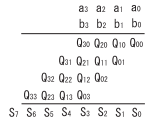
\includegraphics[width=50mm]{mult.png}
		\caption{4bitの乗算の一般形}
	\end{center}
\end{figure}


\begin{figure}[htbp]
	\begin{center}
		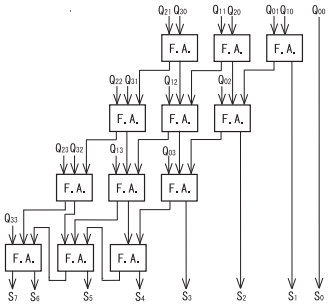
\includegraphics[width=50mm]{mult_full.png}
		\caption{4bit桁上げ保存加算器}
	\end{center}
\end{figure}



\subsection{除算}

\subsubsection{加えもどし法}
被除数から除数を繰り返し引き、引き過ぎたら1 回加算してやる方法である.2進数の場合には1回引けるか否かであって、除数の2の補数
を被除数に加えたとき符号ビットから桁上げがあれば引けたということであり、桁上げがな
ければひけなかったのであるから除数を加え元にもどしてやる。



\section{実験方法}
テキストにある実験課題で与えられた回路を装置を用いて作成し、正しく動作することを真理値表と照らし合わせて確認する.


\section{実験結果}

\subsection{排他的論理和の回路を構成し、正しく動作することを確認せよ.}
排他的論理和の回路を図3のように構成した.


真理値表は表7のようになった.


\begin{figure}[htbp]
	\begin{center}
		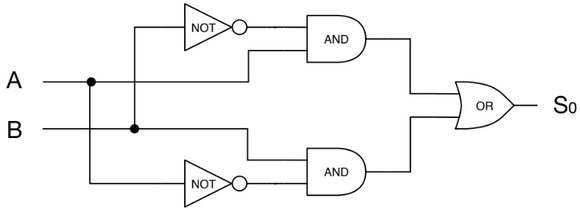
\includegraphics[width=100mm]{work1.png}
		\caption{XORの論理回路}
	\end{center}
\end{figure}



\begin{table}[htbp]
	\caption{実験課題1の真理値表}
	\centering
	\begin{tabular}{|c|c||c|} \hline
    	A & B & $S_0$ \\ \hline \hline
		0 & 0 & 0 \\ \hline
		0 & 1 & 1 \\ \hline
		1 & 0 & 1 \\ \hline
		1 & 1 & 0 \\ \hline
	\end{tabular}
\end{table}

この結果は排他的論理和で期待していた通りの出力であり、正しく動作することを確認することができた.

\subsection{半加算器を構成し、正しく動作することを確認せよ.}
半加算器の回路を図4のように構成した.

真理値表は表8のようになった.

\begin{figure}[htbp]
	\begin{center}
		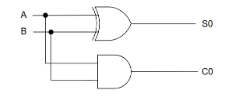
\includegraphics[width=100mm]{half_adder.png}
		\caption{半加算器の論理回路}
	\end{center}
\end{figure}


\begin{table}[htbp]
	\caption{実験課題2の真理値表}
	\centering
	\begin{tabular}{|c|c||c|c|} \hline
		A & B & $S_0$ & $C_0$ \\ \hline \hline
		0 & 0 & 0 & 0 \\ \hline
		0 & 1 & 1 & 0 \\ \hline
		1 & 0 & 1 & 0 \\ \hline
		1 & 1 & 0 & 1 \\ \hline
	\end{tabular}
\end{table}

この結果は半加算器で期待していた通りの出力であり、正しく動作することを確認することができた.

\subsection{全加算器を構成し、正しく動作することを確認せよ.}
全加算器の回路を図5のように構成した.ここで、先程作成した半加算器を利用した.
真理値表は表9のようになった.

\begin{figure}[htbp]
	\begin{center}
		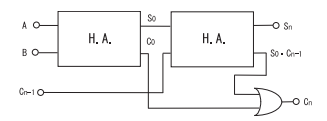
\includegraphics[width=100mm]{full_adder.png}
		\caption{全加算器の論理回路}
	\end{center}
\end{figure}


\begin{table}[htbp]
	\caption{実験課題3の真理値表}
	\centering
	\begin{tabular}{|c|c|c||c|c|} \hline
		A & B & $C_{n-1}$ & $S_n$ & $C_n$ \\ \hline \hline
		0 & 0 & 0 & 0 & 0 \\ \hline
		0 & 0 & 1 & 1 & 0 \\ \hline
		0 & 1 & 0 & 1 & 0 \\ \hline
		0 & 1 & 1 & 0 & 1 \\ \hline
		1 & 0 & 0 & 1 & 0 \\ \hline
		1 & 0 & 1 & 0 & 1 \\ \hline
		1 & 1 & 0 & 0 & 1 \\ \hline
		1 & 1 & 1 & 1 & 1 \\ \hline
	\end{tabular}
\end{table}



この結果は全加算器で期待していた通りの出力であり、正しく動作することを確認することができた.


\subsection{2ビットの全加算器を設計し、正しく動作することを確認せよ.ただし、最下位
桁については半可算器を用いてよい.}

2ビットの全加算器回路を図6のように構成した.ここで、作成した半加算器と全加算器を利用した.
真理値表は表10のようになった.

\begin{figure}[htbp]
	\begin{center}
		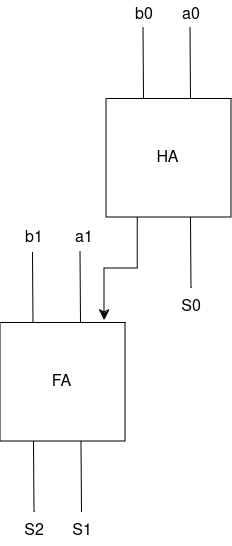
\includegraphics[width=40mm]{2bitadd.png}
		\caption{2bit全加算器の論理回路}
	\end{center}
\end{figure}


\begin{table}[htbp]
	\caption{実験課題4の真理値表}
	\centering
	\begin{tabular}{|c|c|c|c||c|c|c|} \hline
		$a_0$ & $a_1$ & $b_0$ & $b_1$ & $S_0$ & $S_1$ & $S_2$ \\ \hline \hline
		0 & 0 & 0 & 0 & 0 & 0 & 0 \\ \hline
		0 & 0 & 0 & 1 & 0 & 1 & 0 \\ \hline
		0 & 0 & 1 & 0 & 1 & 0 & 0 \\ \hline
		0 & 0 & 1 & 1 & 1 & 1 & 0 \\ \hline
		0 & 1 & 0 & 0 & 0 & 1 & 0 \\ \hline
		0 & 1 & 0 & 1 & 0 & 0 & 1 \\ \hline
		0 & 1 & 1 & 0 & 1 & 1 & 0 \\ \hline
		0 & 1 & 1 & 1 & 1 & 0 & 1 \\ \hline
		1 & 0 & 0 & 0 & 1 & 0 & 0 \\ \hline
		1 & 0 & 0 & 1 & 1 & 1 & 0 \\ \hline
		1 & 0 & 1 & 0 & 0 & 1 & 0 \\ \hline
		1 & 0 & 1 & 1 & 0 & 0 & 1 \\ \hline
		1 & 1 & 0 & 0 & 1 & 1 & 0 \\ \hline
		1 & 1 & 0 & 1 & 1 & 0 & 1 \\ \hline
		1 & 1 & 1 & 0 & 0 & 0 & 1 \\ \hline
		1 & 1 & 1 & 1 & 0 & 1 & 1 \\ \hline
	\end{tabular}
\end{table}


この結果は2bitの全加算器で期待していた通りの出力であり、正しく動作することを確認することができた.


\subsection{全減算器を設計し、正しく動作することを確認せよ.}
全減算器の回路を図7のように構成した.
真理値表は表11のようになった.

\begin{figure}[htbp]
	\begin{center}
		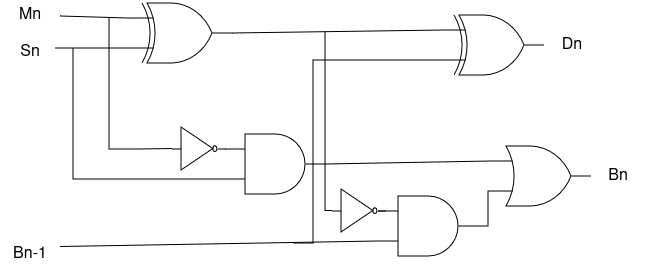
\includegraphics[width=100mm]{sub.png}
		\caption{全減算器の論理回路}
	\end{center}
\end{figure}


\begin{table}[htbp]
	\caption{実験課題5の真理値表}
	\centering
	\begin{tabular}{|c|c|c||c|c|} \hline
		$M_n$ & $S_n$ & $B_{n-1}$ & $D_n$ & $B_n$ \\ \hline \hline
		0 & 0 & 0 & 0 & 0 \\ \hline
		0 & 0 & 1 & 1 & 1 \\ \hline
		0 & 1 & 0 & 1 & 1 \\ \hline
		0 & 1 & 1 & 0 & 1 \\ \hline
		1 & 0 & 0 & 1 & 0 \\ \hline
		1 & 0 & 1 & 0 & 0 \\ \hline
		1 & 1 & 0 & 0 & 0 \\ \hline
		1 & 1 & 1 & 1 & 1 \\ \hline
	\end{tabular}
\end{table}


この結果は減算器で期待していた通りの出力であり、正しく動作することを確認することができた.

\subsection{2ビットの減算器を設計し、正しく動作することを確認せよ.}

2ビットの減算器の回路を図8のように構成した.
真理値表は表12のようになった.

\begin{figure}[htbp]
	\begin{center}
		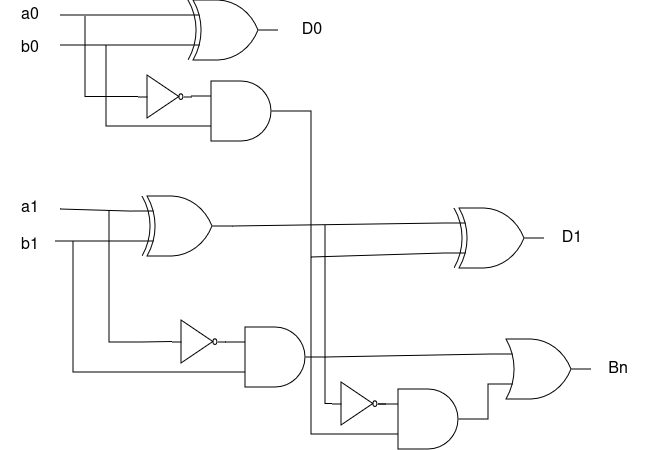
\includegraphics[width=100mm]{2bitsub.png}
		\caption{2bit減算器の論理回路}
	\end{center}
\end{figure}



\begin{table}[htbp]
	\caption{実験課題6の真理値表}
	\centering
	\begin{tabular}{|c|c|c|c||c|c|c|} \hline
		$a_1$ & $a_0$ & $b_1$ & $b_0$ & $D_0$ & $D_1$ & $B_n$ \\ \hline \hline
		0 & 0 & 0 & 0 & 0 & 0 & 0 \\ \hline
		0 & 0 & 0 & 1 & 1 & 1 & 1 \\ \hline
		0 & 0 & 1 & 0 & 0 & 1 & 1 \\ \hline
		0 & 0 & 1 & 1 & 1 & 0 & 1 \\ \hline
		0 & 1 & 0 & 0 & 1 & 0 & 0 \\ \hline
		0 & 1 & 0 & 1 & 0 & 0 & 0 \\ \hline
		0 & 1 & 1 & 0 & 1 & 1 & 1 \\ \hline
		0 & 1 & 1 & 1 & 0 & 1 & 1 \\ \hline
		1 & 0 & 0 & 0 & 0 & 1 & 0 \\ \hline
		1 & 0 & 0 & 1 & 1 & 0 & 0 \\ \hline
		1 & 0 & 1 & 0 & 0 & 0 & 0 \\ \hline
		1 & 0 & 1 & 1 & 1 & 1 & 1 \\ \hline
		1 & 1 & 0 & 0 & 1 & 1 & 0 \\ \hline
		1 & 1 & 0 & 1 & 0 & 1 & 0 \\ \hline
		1 & 1 & 1 & 0 & 1 & 0 & 0 \\ \hline
		1 & 1 & 1 & 1 & 0 & 0 & 0 \\ \hline
	\end{tabular}
\end{table}


この結果は2bitの減算器で期待していた通りの出力であり、正しく動作することを確認することができた.

\subsection{2ビットの乗算器を設計し、正しく動作することを確認せよ.}
2ビットの乗算器の回路を図9のように構成した.
真理値表は表13のようになった.

\begin{figure}[htbp]
	\begin{center}
		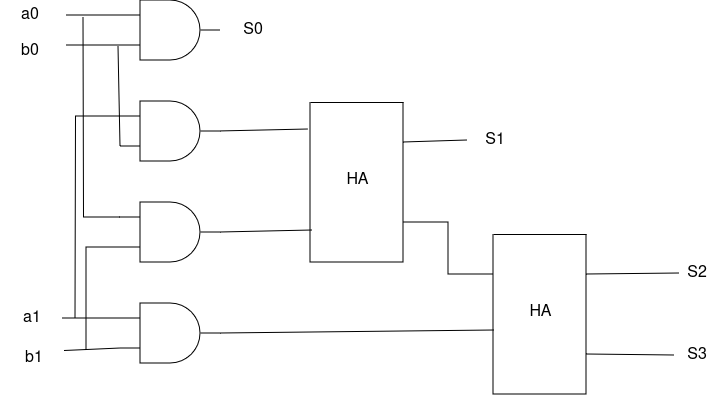
\includegraphics[width=100mm]{2bitmult.png}
		\caption{2bit乗算器の論理回路}
	\end{center}
\end{figure}



\begin{table}[htbp]
	\caption{実験課題7の真理値表}
	\centering
	\begin{tabular}{|c|c|c|c||c|c|c|c|} \hline
		$a_1$ & $a_0$ & $b_1$ & $b_0$ & $S_3$ & $S_2$ & $S_1$ & $S_0$ \\ \hline \hline
		0 & 0 & 0 & 0 & 0 & 0 & 0 & 0 \\ \hline
		0 & 0 & 0 & 1 & 0 & 0 & 0 & 0 \\ \hline
		0 & 0 & 1 & 0 & 0 & 0 & 0 & 0 \\ \hline
		0 & 0 & 1 & 1 & 0 & 0 & 0 & 0 \\ \hline
		0 & 1 & 0 & 0 & 0 & 0 & 0 & 0 \\ \hline
		0 & 1 & 0 & 1 & 0 & 0 & 0 & 1 \\ \hline
		0 & 1 & 1 & 0 & 0 & 0 & 1 & 0 \\ \hline
		0 & 1 & 1 & 1 & 0 & 0 & 1 & 1 \\ \hline
		1 & 0 & 0 & 0 & 0 & 0 & 0 & 0 \\ \hline
		1 & 0 & 0 & 1 & 0 & 0 & 1 & 0 \\ \hline
		1 & 0 & 1 & 0 & 0 & 1 & 0 & 0 \\ \hline
		1 & 0 & 1 & 1 & 0 & 1 & 1 & 0 \\ \hline
		1 & 1 & 0 & 0 & 0 & 0 & 0 & 0 \\ \hline
		1 & 1 & 0 & 1 & 0 & 0 & 1 & 1 \\ \hline
		1 & 1 & 1 & 0 & 0 & 1 & 1 & 0 \\ \hline
		1 & 1 & 1 & 1 & 1 & 0 & 0 & 1 \\ \hline
	\end{tabular}
\end{table}


この結果は2bitの減算器で期待していた通りの出力であり、正しく動作することを確認することができた.




\subsection{2進数の除算の一例を加えもどし法で行い、レポート上で考察せよ。}
例で示された$1235 \div 45$を2進数で、加え戻し方によって実行する.ただし、ここでの除算は1235の2進数表現は11bitとなるから、11bitの被演算子同士で行う.ここで、1235を2進数で表現すると10011010011となり、
45を2進数で表現すると00000101101となる.さらに、45の2進数の補数表現は11111010011となる.
加え戻し方で除算を行うため、10011010011に11111010011を桁上げがなくなるまで繰り返し足していく.
以下はPythonによって生成した結果である.

1回目: 10011010011 + 11111010011 = (1)10010100110 \\
2回目: 10010100110 + 11111010011 = (1)10001111001 \\
3回目: 10001111001 + 11111010011 = (1)10001001100 \\
4回目: 10001001100 + 11111010011 = (1)10000011111 \\
5回目: 10000011111 + 11111010011 = (1)01111110010 \\
6回目: 01111110010 + 11111010011 = (1)01111000101 \\
7回目: 01111000101 + 11111010011 = (1)01110011000 \\
8回目: 01110011000 + 11111010011 = (1)01101101011 \\
9回目: 01101101011 + 11111010011 = (1)01100111110 \\
10回目: 01100111110 + 11111010011 = (1)01100010001 \\
11回目: 01100010001 + 11111010011 = (1)01011100100 \\
12回目: 01011100100 + 11111010011 = (1)01010110111 \\
13回目: 01010110111 + 11111010011 = (1)01010001010 \\
14回目: 01010001010 + 11111010011 = (1)01001011101 \\
15回目: 01001011101 + 11111010011 = (1)01000110000 \\
16回目: 01000110000 + 11111010011 = (1)01000000011 \\
17回目: 01000000011 + 11111010011 = (1)00111010110 \\
18回目: 00111010110 + 11111010011 = (1)00110101001 \\
19回目: 00110101001 + 11111010011 = (1)00101111100 \\
20回目: 00101111100 + 11111010011 = (1)00101001111 \\
21回目: 00101001111 + 11111010011 = (1)00100100010 \\
22回目: 00100100010 + 11111010011 = (1)00011110101 \\
23回目: 00011110101 + 11111010011 = (1)00011001000 \\
24回目: 00011001000 + 11111010011 = (1)00010011011 \\
25回目: 00010011011 + 11111010011 = (1)00001101110 \\
26回目: 00001101110 + 11111010011 = (1)00001000001 \\
27回目: 00001000001 + 11111010011 = (1)00000010100 \\
28回目: 00000010100 + 11111010011 = 11111100111

1回だけ余分に引いてしまっているのだから、最後の結果に45の2進数である00000101101を足す.
$11111100111 + 00000101101 = (1)00000010100$
これは、10進数へ変換すると20である.
これらの結果から、$1235 \div 45 = 27 \cdots 20$ であり、さらに、正しく計算できていることが確認できた.

\subsection{3ビットの比較器を設計し、レポート上に回路図を書け.}
3bitの比較2数$A = A_2 A_1 A_0$, $B = B_2 B_1 B_0$の大小関係について考える.

(i)$A = B$ となるのは、$A_2 = B_2$,$A_1 = B_1$,$A_0 = B_0$のときのみ

(ii)$A > B$ となるのは、$A_2 > B_2$ または$A_2 = B_2, A_1 > B_1$または$A_2 = B_2, A_1 = B_1, A_0 > B_0$

(iii)$A < B$ となるのは、$A_2 < B_2$ または$A_2 = B_2, A_1 < B_1$または$A_2 = B_2, A_1 = B_1, A_0 < B_0$


ここで、1bitの比較器を利用する(図10).1bit比較器をCOMPとすることにする$f_0, f_1, f_2$は(1),(2),(3)と同様に定義した.
これを利用して3bitの比較器を設計した(図11).


\begin{figure}[htbp]
	\begin{center}
		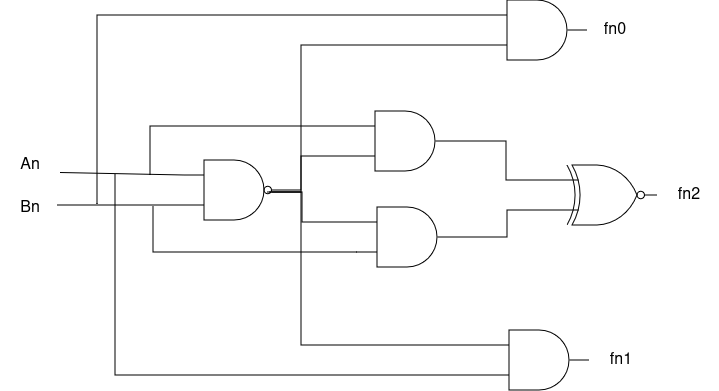
\includegraphics[width=100mm]{1bitcomp.png}
		\caption{1bit比較器の論理回路}
	\end{center}
\end{figure}


\begin{figure}[htbp]
	\begin{center}
		
\includegraphics[width=100mm]{3bitcomp.png}
		\caption{3bit比較器の論理回路}
	\end{center}
\end{figure}




\section{考察}

\subsection{XOR}
今回の実験では様々な回路を設計したがXORを利用する機械が多数あった.例として、半加算器の和の部分をあげる.0と0の和は0,
0と1の和は1,1と1の和は0となり、XORの論理回路における重要性について理解することができた.

\subsection{加算器}
半加算器は下位bitからの繰り上げを考慮しないので足し算における1bit目の和を求める際に有用であることがわかった.
また、全加算器は2bit目以降の和を求める際に必要であることも理解することができた.
さらに、半加算器と全加算器を組み合わせることで2bit以上の加算も今回の実験課題から拡張して行えることがわかった.

\subsection{減算器}
減算器も加算器と同様に、半減算器と全減算器を組み合わせることによって2bit以上の減算器を設計することができることがわかった.
また、論理関数も加算のときに比べても大きな違いはないことがわかった.

\subsection{乗算器}
2 ビット乗算器を実装した.今回の乗算の方法は筆算を行うときと同様に考えるものであり、
部分積を加算することで積を求めた.部分積を加算するために加算器を利用する必要があったが.
2bitの乗算の場合には半加算器を2つ使うことで設計することができた.
しかし、2bitよりも大きいビット数の乗算では全加算器を使う必要があることがわかった.

\subsection{加え戻し法}
加え戻し法は基本的に引き算と商の調整を繰り返すだけなので、手順がシンプルで理解しやすい.
しかし、商の仮定と修正を繰り返すため、計算に時間がかかることがある.
特に被除数が大きな数や除数が小さい計算の場合には、繰り返しの数が多くなってしまうため効率が悪くなることがある.


\subsection{比較器}
加算や減算、乗算だけでなく比較においても簡単な回路の組み合わせによって回路を設計することができることがわかった.
しかし、今回3bitの比較器を設計したが入力の1bitごとの比較を行う必要があり、想定していた以上に回路が複雑になってしまった.


\section{参考文献}
[1]群馬大学 情報科学実験Iテキスト2024年




\end{document}
